% Online sync refresh: revised workshop report, 2026-08-29. figure-path-fix
The supplied $\epsilon$-greedy implementation was extended using the
multi-horizon numerical procedure proposed in
Algorithm~\ref{alg:q2-sublinear-test}. For each selected action $A_t$,
the instantaneous pseudo-regret was evaluated as
\[
    R^\ast-q^\ast(A_t),
\]
where $q^\ast$ was used only for post-action performance evaluation and was
not available to the learning algorithm.

The six exploration schedules considered were
\[
\begin{aligned}
    &\epsilon_t=0, \qquad
    \epsilon_t=0.01, \qquad
    \epsilon_t=0.10,\\
    &\epsilon_t=
    \min\left\{
        \left(
            \frac{k\log(t+1)}{t+1}
        \right)^{1/3},
        1
    \right\},\\
    &\epsilon_t=0.99^t, \qquad
    \epsilon_t=0.90^t.
\end{aligned}
\]
The $t+1$ form in the polynomial schedule accounts for Python's zero-based
indexing. The final exponential-decay case in the supplied code was also
corrected to use $0.90^t$, consistent with its stated label.

To reduce the risk of mistaking finite-horizon transient behaviour for an
asymptotic trend, each policy was simulated for $M=500$ independent reruns
up to
\[
    T_{\max}=10^5,
\]
with cumulative pseudo-regret recorded at
\[
    T_i\in
    \{10^3,\,3\times10^3,\,10^4,\,3\times10^4,\,10^5\}.
\]
At these horizons, the normalised regret $\widehat{\rho}_{T_i}$,
incremental regret rate $\widehat{s}_i$, and effective regret exponent
$\widehat{\alpha}_i$ defined in Question~2 were evaluated. The first two are
the primary definition-based diagnostics. The effective exponent is a
supplementary local log-log slope and is not used as a necessary or
sufficient test for sublinear regret.

\begin{figure}[H]
    \centering
    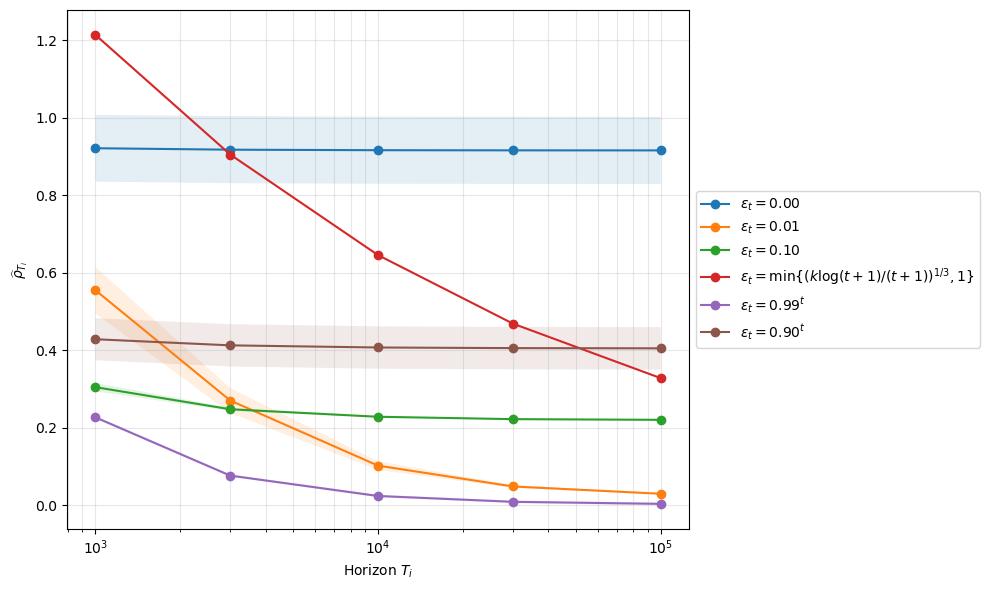
\includegraphics[width=0.92\linewidth]
    {figures/epsilon_multihorizon_normalised_regret.png}
    \caption{Normalised empirical cumulative pseudo-regret
    $\widehat{\rho}_{T_i}$ for the six $\epsilon$-greedy schedules.
    Shaded regions represent approximate 95\% Monte Carlo confidence
    intervals.}
    \label{fig:q3-normalised-regret}
\end{figure}

Figure~\ref{fig:q3-normalised-regret} provides the diagnostic most directly
related to the definition of sublinear regret. The curves for
$\epsilon_t=0$, $\epsilon_t=0.10$, and $\epsilon_t=0.90^t$ clearly approach
positive values and are therefore inconsistent with
$\widehat{\rho}_{T_i}\to0$. The cases $\epsilon_t=0.01$ and
$\epsilon_t=0.99^t$ are less obvious from normalised regret alone because
their curves continue decreasing over the simulated horizons. This motivates
the additional diagnostics introduced in Question~2.

\begin{figure}[H]
    \centering
    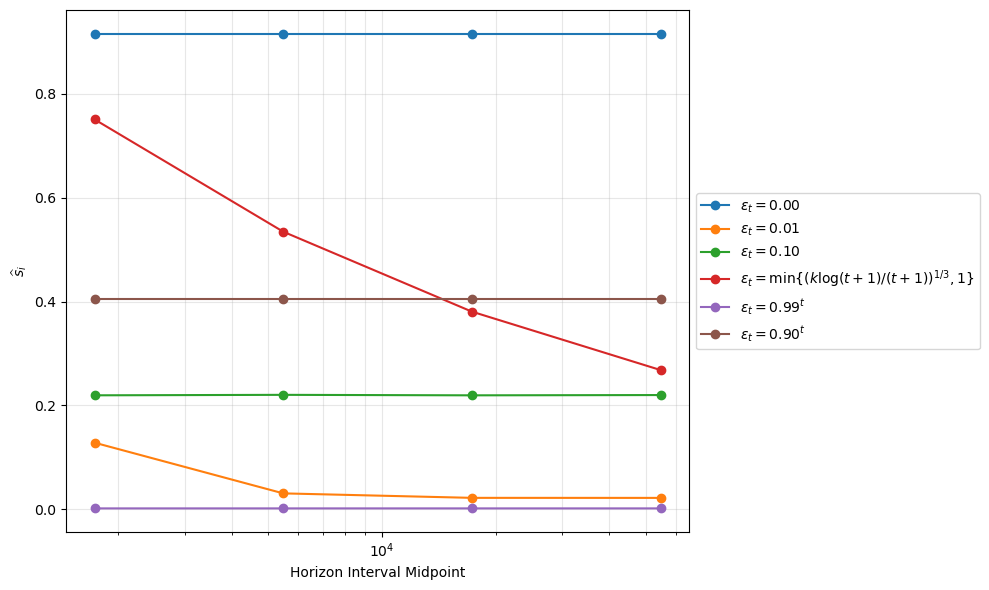
\includegraphics[width=0.92\linewidth]
    {figures/epsilon_incremental_regret_rate.png}
    \caption{Incremental regret rate $\widehat{s}_i$ between consecutive
    simulation horizons.}
    \label{fig:q3-incremental-regret}
\end{figure}

Figure~\ref{fig:q3-incremental-regret} shows whether additional regret is
still accumulating at a non-zero rate. For a linear-regret policy,
$\widehat{s}_i$ should approach a positive constant, whereas for sublinear
regret it should decrease towards zero. The polynomial schedule is the only
case exhibiting persistent decay over all four intervals:
\[
    0.7507
    \;\to\;
    0.5345
    \;\to\;
    0.3805
    \;\to\;
    0.2681.
\]
In contrast, the other schedules eventually exhibit an approximately
constant positive mean incremental regret rate. For $\epsilon_t=0.99^t$,
the corresponding run-level slopes must also be inspected because the mean
is produced by a rare-event mixture.

\begin{figure}[H]
    \centering
    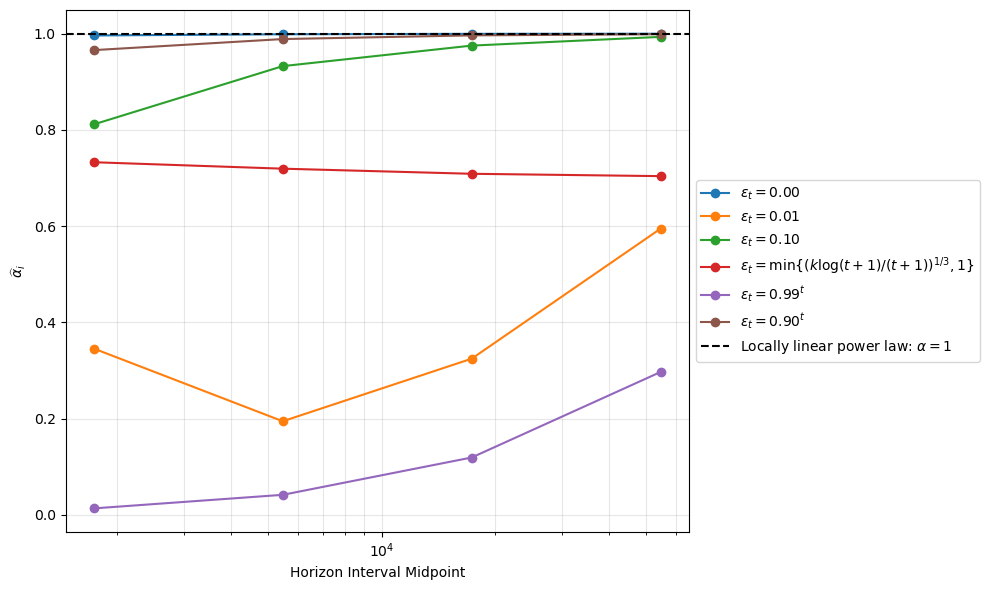
\includegraphics[width=0.92\linewidth]
    {figures/epsilon_effective_regret_exponent.png}
    \caption{Effective regret exponent $\widehat{\alpha}_i$ between
    consecutive horizons. The dashed line $\alpha=1$ corresponds to
    linear power-law growth.}
    \label{fig:q3-effective-exponent}
\end{figure}

The effective exponents in Figure~\ref{fig:q3-effective-exponent} provide a
supplementary indication of the growth order. In particular,
$\widehat{\alpha}_i$ approaches one for several of the policies exhibiting
linear regret, whereas the polynomial schedule remains well below one,
decreasing from approximately $0.733$ to $0.704$. An exponent approaching
one does not by itself prove linear regret: for example, the sublinear
function $T/\log T$ also has a local effective exponent approaching one.

The complete multi-horizon diagnostics are summarised in
Table~\ref{tab:q3-diagnostics}.

\begin{table}[H]
\centering
\caption{Measured multi-horizon numerical diagnostics for the six
$\epsilon$-greedy schedules. Interpretations are given separately in the
text.}
\label{tab:q3-diagnostics}
\resizebox{\textwidth}{!}{
\begin{tabular}{lccc}
\toprule
\textbf{Schedule}
& $\widehat{\rho}_{10^5}$
& $\widehat{s}_1\rightarrow\widehat{s}_4$
& $\widehat{\alpha}_1\rightarrow\widehat{\alpha}_4$ \\
\midrule

$\epsilon_t=0$
& $0.9158$
& $0.9157\to0.9157\to0.9157\to0.9157$
& $0.9963\to0.9988\to0.9996\to0.9999$ \\

$\epsilon_t=0.01$
& $0.0300$
& $0.1282\to0.0306\to0.0220\to0.0219$
& $0.3456\to0.1946\to0.3246\to0.5948$ \\

$\epsilon_t=0.10$
& $0.2207$
& $0.2194\to0.2203\to0.2194\to0.2200$
& $0.8115\to0.9326\to0.9752\to0.9934$ \\

Polynomial decay
& $0.3283$
& $0.7507\to0.5345\to0.3805\to0.2681$
& $0.7329\to0.7195\to0.7089\to0.7040$ \\

$\epsilon_t=0.99^t$
& $0.0040$
& $0.001699\to0.001697\to0.001697\to0.001697$
& $0.0135\to0.0417\to0.1193\to0.2970$ \\

$\epsilon_t=0.90^t$
& $0.4052$
& $0.4049\to0.4049\to0.4049\to0.4049$
& $0.9658\to0.9888\to0.9965\to0.9989$ \\

\bottomrule
\end{tabular}}
\end{table}

Table~\ref{tab:q3-diagnostics} contains measured quantities only. The
following conclusions are manual interpretations of the diagnostic trends,
not outputs of a threshold-based classifier.

For $\epsilon_t=0$, no systematic exploration occurs. The algorithm may
therefore commit permanently to a suboptimal arm. Its incremental regret
rate remains at approximately $0.916$, while
$\widehat{\alpha}_i\to1$, providing clear evidence of linear regret.

For the fixed exploration rate $\epsilon_t=0.10$,
$\widehat{s}_i$ remains almost exactly constant at approximately $0.22$ and
$\widehat{\alpha}_i$ approaches one. Hence, its cumulative regret is clearly
linear. The case $\epsilon_t=0.01$ illustrates why the incremental-rate
diagnostic is useful: although its normalised regret is still decreasing at
$T=10^5$, its incremental regret rate settles at approximately $0.0219$.
Thus the observed behaviour is consistent with a regret curve of the form
\[
    \operatorname{Regret}_T
    \approx
    C+cT,
    \qquad c>0,
\]
where the transient term $C/T$ causes the normalised regret to continue
decreasing before eventually approaching the positive constant $c$.

The polynomial schedule
\[
    \epsilon_t=
    \min\left\{
        \left(
            \frac{k\log(t+1)}{t+1}
        \right)^{1/3},
        1
    \right\}
\]
is the only case that is numerically consistent with sublinear regret.
Its normalised regret continues to decrease, its incremental regret rate
decreases persistently towards zero, and its effective exponent remains
well below one across the largest simulated horizons.

For $\epsilon_t=0.90^t$, exploration decays so rapidly that the algorithm can
become permanently committed to a suboptimal arm. Correspondingly,
$\widehat{s}_i$ approaches the positive value $0.4049$ and
$\widehat{\alpha}_i\to1$, indicating linear regret.

The slower exponential schedule $\epsilon_t=0.99^t$ performs substantially
better at finite horizons, but the multi-horizon test reveals behaviour that
was not apparent in the shorter experiment. Over the final interval
$[30000,100000]$, $499$ of the $500$ reruns have essentially zero individual
late slope, while one rerun has a positive slope of approximately $0.848290$.
Consequently, the mean late slope is
\[
    \widehat{s}_i\approx0.001697,
\]
but this value is a rare-event mixture rather than a precisely estimated
population coefficient. Its effective exponent increases from approximately
$0.014$ to $0.297$ as the horizon grows. Together with the fact that
$\sum_t 0.99^t<\infty$, so exploration can cease before a run identifies the
optimal arm, the result is consistent with a possible linear-regret
component rather than reliable sublinear convergence.

Therefore, among the six tested exploration schedules, the only policy
numerically consistent with sublinear regret is
\[
    \epsilon_t=
    \min\left\{
        \left(
            \frac{k\log(t+1)}{t+1}
        \right)^{1/3},
        1
    \right\}.
\]
The numerical conclusion agrees with the theoretical result that exploration
must decay sufficiently slowly to maintain learning while its long-run
frequency approaches zero. Since only finite horizons and finitely many
reruns are simulated, these results provide numerical evidence of the
asymptotic growth regime rather than a mathematical proof.
